 %%%%%%%%%%%%%%%%%%%%%%%%%%%%%%%%%%%%%%%%%%%%%%%%%%%%%%%%%%%%%%%%%%%%%%
% LaTeX Template: Newsletter  % Source: http://www.howtotex.com
%
% Feel free to distribute this example, but please keep the referral
% to howtotex.com
% Date: September 2011 
%%% ---------------
%%% PREAMBLE
%%% ---------------
\documentclass[10pt,a4paper]{article}

% Define geometry (without using the geometry package)
\setlength\topmargin{-48pt}
\setlength\headheight{13pt}
\setlength\headsep{25pt}
\setlength\marginparwidth{-20pt}
\setlength\textwidth{7.0in}
\setlength\textheight{9.5in}
\setlength\oddsidemargin{-30pt}
\setlength\evensidemargin{-30pt}

\frenchspacing						% better looking spacing

% Call packages we'll need
\usepackage[norsk,english]{babel}			% english
\usepackage{graphicx}				% images
\usepackage{rotating}

\usepackage{caption}
\captionsetup[figure]{font=small}

\usepackage{amssymb,amsmath}		% math
\usepackage{multicol}				% three-column layout
\usepackage{url}					% clickable links
\usepackage{marvosym}				% symbols
\usepackage{wrapfig}				% wrapping text around figures
\usepackage{arev} 
\usepackage[T1]{fontenc}			% https://tex.stackexchange.com/questions/59403/what-font-packages-are-installed-in-tex-live % font encoding https://latexref.xyz/fontenc-package.html
\usepackage{blindtext}				% dummy text
\usepackage{datetime}				% custom date
	\newdateformat{mydate}{\monthname[\THEMONTH] \THEYEAR}
\usepackage[pdfpagemode=FullScreen,
			colorlinks=false]{hyperref}	% links and pdf behaviour

% Customize (header and) footer
\usepackage{fancyhdr}
\pagestyle{fancy}
\lfoot{	\footnotesize 
		RITMO report, Bodies in Concert \\
		\Mundus\ \href{https://www.uio.no/ritmo/english/news-and-events/events/artistic-performances/2023/symphony-experiment/index.html}{Lydo Concerts 2023}	\quad										\quad
		\Letter\ \href{mailto:finn.upham@imv.uio.no}{finn.upham@imv.uio.no}
	  }
\cfoot{}
\rfoot{\footnotesize ~\\ Page \thepage}
\renewcommand{\headrulewidth}{0.1pt}	% no bar on top of page
\renewcommand{\footrulewidth}{0.4pt}	% bar on bottom of page

%%% ---------------
%%% DEFINITIONS
%%% ---------------

% Define separators
\newcommand{\HorRule}[1]{\noindent\rule{\linewidth}{#1}} % Creating a horizontal rule
\newcommand{\SepRule}{\noindent							 % Creating a separator
						\begin{center}
							\rule{250pt}{1pt}
						\end{center}
						}						

% Define Title en News input
\newcommand{\JournalName}[1]{%


		\begin{center}	
		\noindent\raisebox{\dimexpr2.1\baselineskip-\height}{
\includegraphics[height=0.5in]{RITMO-hovedmerke-290818_150px.png}}
			\Huge \usefont{T1}{pag}{m}{n}
			#1%
		\end{center}	
		\par \normalsize \normalfont}

\newcommand{\NewsItem}[1]{%
		\usefont{T1}{pag}{b}{n} 	
		\large #1 \vspace{4pt}
		\par \normalsize \normalfont}
		
\newcommand{\NewsAuthor}[1]{%
			\hfill by \textsc{#1} \vspace{4pt}
			\par \normalfont}		

%%% ---------------
%%% BEGIN DOCUMENT
%%% ---------------
\begin{document}
% Title	
% -----
\JournalName{Bodies in Concert: Performer summary}
\noindent\HorRule{3pt} \\[-0.75\baselineskip]
\HorRule{1pt}
% -----
% Front article
% -----
\vspace{0.5cm}
	\SepRule
\vspace{0.5cm}

\begin{center}
\begin{minipage}[h]{0.75\linewidth}
	\begin{wrapfigure}{l}{0.41\textwidth}
		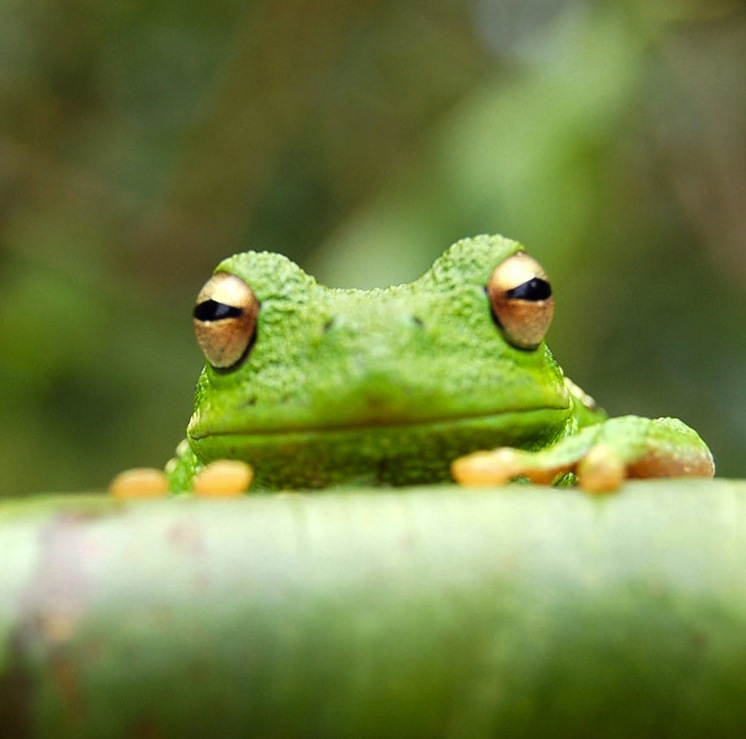
\includegraphics[width=0.42\textwidth]{frog.jpg}
		\\	% this spacer is needed to make the text on the right fit OK
	\end{wrapfigure}
	
	\NewsItem{Frog eats monkey}
	\emph{\blindtext}
\end{minipage}
\end{center}
% -----

%% Other news (1)
% -----
\vspace{0.5cm}
	\SepRule
\vspace{0.5cm}
\begin{multicols}{2}
	\NewsItem{Monkey eats elephant}
	\NewsAuthor{F. Wenneker}
	\blindtext[2] 
% -----

\vspace{1cm}
% Other news (2)
% -----
\NewsItem{Elephant eats frog}
\NewsAuthor{J. Doe}
	\blindtext[1]
		\begin{center}
			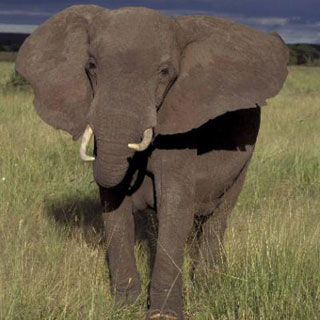
\includegraphics[width=0.8\linewidth]{elephant}
		\end{center}
		\blindtext[1]
\end{multicols}

\section{Trumpet}
 
This document shares some outputs from data collected with the equivitals.
\begin{figure}
\includegraphics[width=\linewidth]{/Users/finn/Desktop/Current_Projects/Stavanger/Summaries/Plots/Waves/Resp_BR602_Tcha_waves.jpg}
\caption{Respiration during each performance of one piece.}
\label{6Resp}
\end{figure}
\end{document}


\clearpage 
\section*{Group signals}
%% Front article

\begin{center}
\begin{minipage}[h]{0.90\linewidth}
	\begin{wrapfigure}{l}{0.6\textwidth}
		\includegraphics[width=0.60\textwidth]{/Users/finn/Desktop/Current_Projects/Stavanger/Signal_Preparation/plots/Synch_taps_C2_Demo.png}
		\\	% this spacer is needed to make the text on the right fit OK
	\end{wrapfigure}
	
	\NewsItem{Synchronisation Taps}
	This figure shows the quantity of motion measured from each participant's physiology sensor in a specific intervals of time, ordered by section. Here it is zoomed into the 30 seconds around the synchronisation taps the orchestra performed during the second Lydo concert, showing the original device time alignment above and the effect of correcting those timings by aligning your taps. (The beginning of Clapping music was also used as a secondary check on signal alignment.) Thank you for tapping along to the beeps! This essential task allows us to study your collective coordination with much greater temporal precision.
	%\emph{\blindtext}
\end{minipage}
\end{center}
% -----
% -----
\vspace{0.5cm}
	\SepRule
\vspace{0.5cm}

Analysis of these measures across performers is ongoing, with many patterns to be discovered. The orchestra is an exceptional example of human coordination, with many bodies simultaneously producing sound with great control and replicability. In the next months, we will carry out different analyses on the performers' data that will show us how they coordinate with the others in the orchestra and how musicians' bodies engage with the music. For example: 
\begin{itemize}
\item \textbf{Performance variability}: We will look at when in the concerts the ensemble played very similarly, and when they were more variable. Our research on small ensembles has found more variablity in moments that are more emotionally expressive. Is this the same for an orchestra, with more people to coordinate?\item \textbf{Inspiration alignment}: When do musicians from different sections breathe together? Entries, accents, section changes,... something in the music is prompting this coordination, even in string players and percussionists.\item \textbf{Rhythmicity and Synchrony with the Conductor}: Conducting gestures change with the rhythmic character of the music, does this translate to different qualities of synchrony across the ensemble? We expect that synchronization is more precise when the music is very rhythmical, but let's see what the data says.
\end{itemize}

 Below are some previews of emergent patterns.
\ % -----
	\SepRule

%\section{Holmenkollen 2023 relay Physio report}
\subsection*{Relay Race participation}
 Alexander Jenseniuns wore an Equivital monitor vest while participated in Holmenkollen 2023 for RITMO, running leg 1: Louisesgate. 
 Alexanders run time was 245.0 s over 1100 m. This report shares some views of his physiological state before, during and after running. 
\begin{figure}[h]
\includegraphics[width=\linewidth]{/Users/finn/Desktop/Current_Projects/Stavanger/Summaries/Plots/Relay/BR607_leg_Relay.png}
\caption{Heart Rate, Respiration wave, Quantity of Motion, and Skin tempurature around the time Alexander was running. Was there some kind of disruption from 17:17:20?}
\label{leg}
\end{figure}
\begin{sidewaysfigure}[h]
\includegraphics[width=\linewidth]{/Users/finn/Desktop/Current_Projects/Stavanger/Summaries/Plots/Relay/BR607_Full_Relay.png}
\caption{For reference, the same measurements over the full duration of the relay race. Notice the temperature rise after the interval of running.}
\label{Full}
\end{sidewaysfigure}
\begin{figure}[h]
\includegraphics[width=\linewidth]{/Users/finn/Desktop/Current_Projects/Stavanger/Summaries/Plots/Relay/BR607_5s_samples_Relay.png}
\caption{To display more clearly the behaviour of these signals in different stats, 5 s samples of raw signals before, during and after his leg. Notice the changing yaxes on respiration and quantity of motion. This pre-run intervals shows typical irregular respiration, the midrun shows manageable noise in the ECG signal. Slower step rate and respiration rate post-run, while still breathing deeply.}
\label{5s}
\end{figure}
\begin{figure}[h]
\includegraphics[width=\linewidth]{/Users/finn/Desktop/Current_Projects/Stavanger/Summaries/Plots/Relay/BR607_resp_phases.png}
\caption{Distributions of Inspiration and Expirations times against depths before, during, and after running. Inspiration/Expiration ratio per breath distinguishes mode of respiration: Before the run, inspiration time is much shorter than irregularly timed expirations. During running, inspiration and expiration are almost even while ventilation is maximised. After the run, inspirations are longer but more stable as breathing continues to be deeper in cool down while expirations slow again.}
\label{resp}
\end{figure}

\end{document}

% -----
\end{document} 
